% !Mode:: "TeX:UTF-8"
\chapter{李群与李代数}
\label{cpt:4}
\begin{mdframed}  
	\textbf{主要目标}
	\begin{enumerate}[labelindent=0em,leftmargin=1.5em]
		\item 理解李群与李代数的概念,掌握$\mathrm{SO}(3), \mathrm{SE}(3)$与对应李代数的表示方式。
		\item 理解BCH近似的意义。
		\item 学会在李代数上的扰动模型。
		\item 使用Sophus对李代数进行运算。
	\end{enumerate}
\end{mdframed} 

上一讲,我们介绍了三维世界中刚体运动的描述方式,包括旋转矩阵、旋转向量、欧拉角、四元数等若干种方式。我们重点介绍了旋转的表示,但是在SLAM中,除了表示之外,我们还要对它们进行估计和优化。因为在SLAM中位姿是未知的,而我们需要解决形如“\textbf{什么样的相机位姿最符合当前观测数据}”这样的问题。一种典型的方式是把它构建成一个优化问题,求解最优的$\bm{R}, \bm{t}$,使得误差最小化。

如前所言,旋转矩阵自身是带有约束的(正交且行列式为1)。它们作为优化变量时,会引入额外的约束,使优化变得困难。通过李群—李代数间的转换关系,我们希望把位姿估计变成无约束的优化问题,简化求解方式。考虑到读者可能还没有李群李代数的基本知识,我们将从最基本的知识开始讲起。
\newpage
\includepdf{resources/other/ch4.pdf}

\newpage 
\section{李群与李代数基础}
上一讲,我们介绍了旋转矩阵和变换矩阵的定义。当时,我们说三维旋转矩阵构成了\textbf{特殊正交群}$\mathrm{SO}(3)$,而变换矩阵构成了\textbf{特殊欧氏群}$\mathrm{SE}(3)$。它们写起来像这样:
\begin{equation}
\mathrm{SO}(3) = \{ \bm{R} \in \mathbb{R}^{3 \times 3} | \bm{R R}^\mathrm{T} = \bm{I}, \det(\bm{R})=1 \}.
\end{equation}
\begin{equation}
\mathrm{SE}(3) = \left\{ \bm{T} = \left[ {\begin{array}{*{20}{c}}
	\bm{R} & \bm{t} \\
	{{\bm{0}^\mathrm{T}}} & 1
	\end{array}} \right]
\in \mathbb{R}^{4 \times 4} | \bm{R} \in \mathrm{SO}(3), \bm{t} \in \mathbb{R}^3\right\}.
\end{equation}

不过,当时我们并未详细解释\textbf{群}的含义。细心的读者应该会注意到,旋转矩阵也好,变换矩阵也好,\textbf{它们对加法是不封闭的}。换句话说,对于任意两个旋转矩阵$\bm{R}_1, \bm{R}_2$,按照矩阵加法的定义,和不再是一个旋转矩阵:
\begin{equation}
\bm{R}_1 + \bm{R}_2  \notin \mathrm{SO}(3), \quad \bm{T}_1 + \bm{T}_2  \notin \mathrm{SE}(3).
\end{equation}
你也可以说两种矩阵并没有良好定义的加法,或者通常矩阵加法对这两个集合不封闭。相对地,它们只有一种较好的运算:乘法。$\mathrm{SO}(3)$和$\mathrm{SE}(3)$关于乘法是封闭的:
\begin{equation}
\bm{R}_1 \bm{R}_2  \in \mathrm{SO}(3), \quad \bm{T}_1 \bm{T}_2  \in \mathrm{SE}(3).
\end{equation}
同时我们也可以对任何一个旋转或变换矩阵(在乘法的意义上)求逆。我们知道,乘法对应着旋转或变换的复合,两个旋转矩阵相乘表示做了两次旋转。对于这种只有一个(良好的)运算的集合,我们称之为\textbf{群}。

\subsection{群}
接下来我们要稍微涉及一些抽象代数方面的知识。我觉得这是讨论李群李代数的必要条件,但实际上除了数学、物理系的同学之外,大部分同学在本科学习中并不会接触到这方面的知识。所以我们先来看一些基本的知识。

群(Group)是\textbf{一种集合}加上\textbf{一种运算}的代数结构。我们把集合记作$A$,运算记作$\cdot$,那么群可以记作$G=(A,\cdot)$。群要求这个运算满足以下几个条件:

\begin{enumerate}
\item { \emph{封闭性}}:$ \quad \forall a_1, a_2 \in A, \quad a_1 \cdot a_2 \in A$.
\item { \emph{结合律}}:$ \quad \forall a_1, a_2, a_3 \in A, \quad (a_1 \cdot a_2) \cdot a_3 = a_1 \cdot ( a_2 \cdot a_3) $.
\item { \emph{幺元}}:$ \quad \exists a_0 \in A, \quad \mathrm{s.t.} \quad \forall a \in A, \quad a_0 \cdot a = a \cdot a_0 = a $.
\item { \emph{逆}}:$ \quad \forall a \in A, \quad \exists a^{-1} \in A, \quad s.t. \quad a \cdot a^{-1} = a_0 $.
\end{enumerate}

读者可以记作“封结幺逆”\footnote{谐音“凤姐咬你”。}。容易验证,旋转矩阵集合和矩阵乘法构成群,同样变换矩阵和矩阵乘法也构成群(因此才能称它们为旋转矩阵群和变换矩阵群)。其他常见的群包括整数的加法$(\mathbb{Z}, +)$,去掉0后的有理数的乘法(幺元为1)$(\mathbb{Q}\backslash 0, \cdot )$,等等。矩阵中常见的群有:

\begin{itemize}
\item \emph{一般线性群$\mathrm{GL}(n)$} \quad 指$n \times n$的可逆矩阵,它们对矩阵乘法成群。

\item \emph{特殊正交群$\mathrm{SO}(n)$} \quad 也就是所谓的旋转矩阵群,其中$\mathrm{SO}(2)$ 和$\mathrm{SO}(3)$最为常见。

\item \emph{特殊欧氏群$\mathrm{SE}(n)$} \quad 也就是前面提到的$n$维欧氏变换,如$\mathrm{SE}(2)$和$\mathrm{SE}(3)$。
\end{itemize}

群结构保证了在群上的运算具有良好的性质,群论则是研究群的各种结构和性质的理论。对群论感兴趣的读者可以参考任意一本近世代数教材。\textbf{李群}是指具有连续(光滑)性质的群。像整数群$\mathbb{Z}$那样离散的群没有连续性质,所以不是李群。而$\mathrm{SO}(n)$和$\mathrm{SE}(n)$在实数空间上是连续的。我们能够直观地想象一个刚体能够连续地在空间中运动,所以它们都是李群。由于$\mathrm{SO}(3)$和$\mathrm{SE}(3)$对于相机姿态估计尤其重要,所以我们主要讨论这两个李群。然而,严格地讨论“连续”、“光滑”这些概念需要具备分析和拓扑学的知识,但我们不是数学书,所以只介绍一些重要的、与SLAM直接相关的结论。如果读者对李群的理论性质感兴趣,请参考文献\cite{Varadarajan2013}。

李群与李代数通常有两种思路来介绍。一是直接引入李群和李代数,然后告诉读者每个李群对应着一个李代数之类的事实,但这样的话,读者会觉得李代数似乎是一个从天而降的符号,不知道它有什么物理意义。所以,我准备稍微花一点时间从旋转矩阵引出李代数,类似于文献\cite{Ma2012}的做法。我们先从较简单的$\mathrm{SO}(3)$开始讨论,引出$\mathrm{SO}(3)$上面的李代数$\mathfrak{so}(3)$。

\subsection{李代数的引出}
考虑任意旋转矩阵$\bm{R}$,我们知道它满足:
\begin{equation}
\bm{R} \bm{R}^\mathrm{T}=\bm{I}.
\end{equation}
现在,我们说,$\bm{R}$是某个相机的旋转,它会随时间连续地变化,即为时间的函数:$\bm{R}(t)$。由于它仍是旋转矩阵,有
\[
\bm{R}(t) \bm{R}(t) ^T = \bm{I}.
\]
在等式两边对时间求导,得到:
\[
\bm{\dot{R}} (t) \bm{R} {(t)^\mathrm{T}} + \bm{R} (t) \bm{\dot{R}} {(t)^\mathrm{T}} = 0.
\]
整理得:
\begin{equation}
\bm{\dot{R}} (t) \bm{R} {(t)^\mathrm{T}} = - \left(  \bm{\dot{R}} (t) \bm{R} {(t)^\mathrm{T}} \right)^\mathrm{T} .
\end{equation}

可以看出$\bm{\dot{R}} (t) \bm{R} {(t)^\mathrm{T}}$是一个\textbf{反对称}矩阵。回忆一下,我们在式\eqref{eq:cross}介绍叉积时,引入了$^\wedge$符号,将一个向量变成了反对称矩阵。同理,对于任意反对称矩阵,我们亦能找到唯一一个与之对应的向量。把这个运算用符号$^{\vee}$表示:
\begin{equation}
{\bm{a}^ \wedge } = \bm{A} = \left[ {\begin{array}{*{20}{c}}
	0&{ - {a_3}}&{{a_2}}\\
	{{a_3}}&0&{ - {a_1}}\\
	{ - {a_2}}&{{a_1}}&0
	\end{array}} \right], \quad 
{ \bm{A}^ \vee } = \bm{a}.
\end{equation}

于是,由于$\bm{\dot{R}} (t) \bm{R} {(t)^\mathrm{T}}$是一个反对称矩阵,我们可以找到一个三维向量$\boldsymbol{\phi} (t) \in \mathbb{R}^3$与之对应:
\[
  \bm{ \dot{R} } (t) \bm{R}(t)^\mathrm{T} = \boldsymbol{\phi} (t) ^ {\wedge}.
\]

等式两边右乘$\bm{R}(t)$,由于$\bm{R}$为正交阵,有:
\begin{equation}
\label{eq:dR}
  \bm{ \dot{R} } (t)  = \boldsymbol{\phi} (t)^{\wedge} \bm{R}(t) = 
 \left[ {\begin{array}{*{20}{c}}
  	0&{ - {\phi _3}}&{{\phi _2}}\\
  	{{\phi _3}}&0&{ - {\phi _1}}\\
  	{ - {\phi _2}}&{{\phi _1}}&0
  	\end{array}} \right] \bm{R} (t).
\end{equation}

可以看到,每对旋转矩阵求一次导数,只需左乘一个$\boldsymbol{\phi}^\wedge (t)$矩阵即可。考虑$t_0=0$时刻,设此时旋转矩阵为$\bm{R}(0) = \bm{I}$。按照导数定义,可以把$\bm{R}(t)$在$t=0$附近进行一阶泰勒展开:
\begin{equation}
\begin{aligned}
\bm{R} \left( t \right) & \approx \bm{R} \left( t_0 \right) + \dot {\bm{R}} \left( {{t_0}} \right)\left( {t - {t_0}} \right)\\
&= \bm{I} + \boldsymbol{\phi} {\left( {{t_0}} \right)^ \wedge } \left( t \right).
\end{aligned}
\end{equation}

我们看到$\boldsymbol{\phi}$反映了$\bm{R}$的导数性质,故称它在$\mathrm{SO}(3)$原点附近的正切空间(Tangent Space)上。同时在$t_0$附近,设$\boldsymbol{\phi}$保持为常数$\boldsymbol{\phi}(t_0) = \boldsymbol{\phi}_0$。那么根据式\eqref{eq:dR},有:
\[
\bm{ \dot{R} } (t) = \boldsymbol{\phi} (t_0) ^ {\wedge} \bm{R}(t) = \boldsymbol{\phi}_0^ {\wedge} \bm{R}(t).
\]

上式是一个关于$\bm{R}$的微分方程,而且有初始值$\bm{R}(0) = \bm{I}$,解之,得:
\begin{equation}
\label{eq:so3ode}
\bm{R}(t) = \exp \left( \boldsymbol{\phi}_0^\wedge t \right).
\end{equation}

读者可以验证上式对微分方程和初始值均成立。这说明在$t = 0$附近,旋转矩阵可以由$\exp \left( \boldsymbol{\phi}_0^\wedge t \right)$计算出来\footnote{此时我们还没有说明$\exp$是如何作用的。我们马上会看到它的定义和计算过程。}。我们看到,旋转矩阵$\bm{R}$与另一个反对称矩阵$\boldsymbol{\phi}_0^\wedge t$通过指数关系发生了联系。但是矩阵的指数是什么呢?这里我们有两个问题需要澄清:

\begin{enumerate}
	\item 给定某时刻的$\bm{R}$,我们就能求得一个$\boldsymbol{\phi}$,它描述了$\bm{R}$在局部的导数关系。与$\bm{R}$对应的$\boldsymbol{\phi}$有什么含义呢?我们说,$\boldsymbol{\phi}$正是对应到$\mathrm{SO}(3)$上的李代数$\mathfrak{so}(3)$;
	\item 其次,给定某个向量$\boldsymbol{\phi}$时,矩阵指数$\exp (\boldsymbol{\phi} ^\wedge )$如何计算?反之,给定$\bm{R}$时,能否有相反的运算来计算$\boldsymbol{\phi}$?事实上,这正是李群与李代数间的指数/对数映射。
\end{enumerate}

下面我们来解决这两个问题。
\subsection{李代数的定义}
每个李群都有与之对应的李代数。李代数描述了李群的局部性质,准确地说,是单位元附近的正切空间。一般的李代数的定义如下:

李代数由一个集合$\mathbb{V}$,一个数域$\mathbb{F}$和一个二元运算$[,]$组成。如果它们满足以下几条性质,则称$(\mathbb{V}, \mathbb{F}, [,])$ 为一个李代数,记作$\mathfrak{g}$。

\begin{enumerate}
	\item{ \emph{封闭性} } \quad $\forall \bm{X}, \bm{Y} \in \mathbb{V}, [\bm{X}, \bm{Y}] \in \mathbb{V}$.
	\item{ \emph{双线性} } \quad $\forall \bm{X},\bm{Y},\bm{Z} \in \mathbb{V}, a,b \in \mathbb{F}, $ 有:
	\[
	[a\bm{X}+b\bm{Y}, \bm{Z}] = a[\bm{X}, \bm{Z}] + b [ \bm{Y}, \bm{Z} ], \quad [\bm{Z}, a \bm{X}+b\bm{Y}] = a [\bm{Z}, \bm{X} ]+ b [\bm{Z},\bm{Y}] .
	\]
	\item{ \emph{自反性}}\footnote{自反性是指自己与自己的运算为零。} \quad $\forall \bm{X} \in \mathbb{V}, [\bm{X},\bm{X}] = \bm{0}$.
	\item { \emph{雅可比等价} } \quad $\forall \bm{X},\bm{Y},\bm{Z} \in \mathbb{V}, [\bm{X}, [\bm{Y},\bm{Z}] ] + [\bm{Z}, [\bm{X},\bm{Y}] ] + [\bm{Y}, [\bm{Z},\bm{X}]] =\bm{0}$.
\end{enumerate}
其中二元运算被称为\textbf{李括号}。从表面上来看,李代数所需要的性质还是挺多的。相比于群中的较为简单的二元运算,李括号表达了两个元素的差异。它不要求结合律,而要求元素和自己做李括号之后为零的性质。作为例子,三维向量$\mathbb{R}^3$ 上定义的叉积$\times$是一种李括号,因此$\mathfrak{g} = (\mathbb{R}^3, \mathbb{R}, \times)$构成了一个李代数。读者可以尝试将叉积的性质代入到上面四条性质中。

\subsection{李代数$\mathfrak{so}(3)$}
之前提到的$\boldsymbol{\phi}$,事实上是一种李代数。$\mathrm{SO}(3)$对应的李代数是定义在$\mathbb{R}^3$上的向量,我们记作$\boldsymbol{\phi}$。根据前面的推导,每个$\boldsymbol{\phi}$都可以生成一个反对称矩阵:
\begin{equation}
\label{eq:phi}
\boldsymbol{\varPhi} = \boldsymbol{\phi}^{\wedge} = \left[ {\begin{array}{*{20}{c}}
	0&{ - {\phi _3}}&{{\phi _2}}\\
	{{\phi _3}}&0&{ - {\phi _1}}\\
	{ - {\phi _2}}&{{\phi _1}}&0
	\end{array}} \right] \in \mathbb{R}^{3 \times 3}.
\end{equation}

在此定义下,两个向量$\boldsymbol{\phi}_1, \boldsymbol{\phi}_2$的李括号为
\begin{equation}
[\boldsymbol{\phi}_1, \boldsymbol{\phi}_2] = \left( \bm{ \varPhi }_1 \bm{ \varPhi }_2 - \bm{ \varPhi }_2 \bm{ \varPhi }_1 \right)^\vee.
\end{equation}

读者可以验证该定义下的李括号满足上面的几条性质。由于向量$\boldsymbol{\phi}$与反对称矩阵是一一对应的,在不引起歧义的情况下,就说$\mathfrak{so}(3)$的元素是三维向量或者三维反对称矩阵,不加区别:
\begin{equation}
\mathfrak{so}(3) = \left\{ \boldsymbol{\phi} \in \mathbb{R}^3, \boldsymbol{\varPhi} = \boldsymbol{\phi^\wedge} \in \mathbb{R}^{3 \times 3} \right\}.
\end{equation}
有些书里也会用$\widehat{\boldsymbol{\phi}}$这样的符号表示反对称,但意义是一样的。至此,我们已清楚了$\mathfrak{so}(3)$的内容。它们是一个由\textbf{三维向量}组成的集合,每个向量对应到一个反对称矩阵,可以用于表达旋转矩阵的导数。它与$\mathrm{SO}(3)$的关系由指数映射给定:
\begin{equation}
\bm{R} = \exp ( \boldsymbol{\phi}^\wedge ).
\end{equation}
指数映射会在稍后介绍。由于已经介绍了$\mathfrak{so}(3)$,我们顺带先来看$\mathrm{SE}(3)$上对应的李代数。

\subsection{李代数$\mathfrak{se}(3)$}
对于$\mathrm{SE}(3)$,它也有对应的李代数$\mathfrak{se}(3)$。为节省篇幅,这里就不介绍如何引出$\mathfrak{se}(3)$了。与$\mathfrak{so}(3)$相似,$\mathfrak{se}(3)$位于$\mathbb{R}^6$空间中:
\begin{equation}
\mathfrak{se}(3) = \left\{ { \boldsymbol{\xi}  = \left[ \begin{array}{l}
	\boldsymbol{\rho} \\
	\boldsymbol{\phi} 
	\end{array} \right]
	 \in { \mathbb{R}^6} ,
	 \boldsymbol{\rho}  \in { \mathbb{R}^3}, \boldsymbol{\phi}  \in \mathfrak{so} \left( 3 \right),{ \boldsymbol{\xi} ^ \wedge } = \left[ {\begin{array}{*{20}{c}}
		{{ \boldsymbol{\phi} ^ \wedge }}& \boldsymbol{\rho} \\
		{{\bm{0}^\mathrm{T}}}&0
		\end{array}} \right] \in { \mathbb{R}^{4 \times 4}}} \right\}.
\end{equation}
我们把每个$\mathfrak{se}(3)$元素记作$\boldsymbol{\xi}$,它是一个六维向量。前三维为平移(但含义与变换矩阵中的平移不同,分析见后),记作$\boldsymbol{\rho}$;后三维为旋转,记作$\boldsymbol{\phi}$,实质上是$\mathfrak{so}(3)$元素\footnote{请注意有些地方把旋转放前面,平移放后面,也是可行的。在程序里则无所谓前后,它们都存储在一个结构体中。}。同时,我们拓展了$^\wedge$符号的含义。在$\mathfrak{se}(3)$中,同样使用$^\wedge$符号,将一个六维向量转换成四维矩阵,但这里不再表示反对称:
\begin{equation}
{ \boldsymbol{\xi} ^ \wedge } = \left[ {\begin{array}{*{20}{c}}
	{{ \boldsymbol{\phi} ^ \wedge }}& \boldsymbol{\rho} \\
	{{\bm{0}^\mathrm{T}}}&0
	\end{array}} \right] \in { \mathbb{R}^{4 \times 4}}.
\end{equation}

我们仍使用$^\wedge$和$^\vee$符号来指代“从向量到矩阵”和“从矩阵到向量”的关系,以保持和$\mathfrak{so}(3)$上的一致性。它们依旧是一一对应的。读者可以简单地把$\mathfrak{se}(3)$理解成“由一个平移加上一个$\mathfrak{so}(3)$元素构成的向量”(尽管这里的$\boldsymbol{\rho}$还不直接是平移)。同样,李代数$\mathfrak{se}(3)$亦有类似于$\mathfrak{so}(3)$的李括号:
\begin{equation}
[ \boldsymbol{\xi}_1, \boldsymbol{\xi}_2 ] = \left( \boldsymbol{\xi}_1^\wedge \boldsymbol{\xi}_2^\wedge -\boldsymbol{\xi}_2^\wedge \boldsymbol{\xi}_1^\wedge \right) ^\vee.
\end{equation}

读者可以验证它是否满足李代数的定义(留作习题)。至此我们已经见过两种重要的李代数$\mathfrak{so}(3)$和$\mathfrak{se}(3)$了。

\section{指数与对数映射}

\subsection{$\mathrm{SO}(3)$上的指数映射}

现在来考虑第二个问题:如何计算$\exp ( \boldsymbol{\phi}^{\wedge} )$?显然它是一个矩阵的指数,在李群和李代数中,称为指数映射(Exponential Map)。同样,我们会先讨论$\mathfrak{so}(3)$的指数映射,再讨论$\mathfrak{se}(3)$的情形。

任意矩阵的指数映射可以写成一个泰勒展开,但是只有在收敛的情况下才会有结果,其结果仍是一个矩阵:
\begin{equation}
\exp(\bm{A}) = \sum\limits_{n = 0}^\infty  {\frac{1}{{n!}}{ \bm{A}^n}}.
\end{equation}

同样地,对$\mathfrak{so}(3)$中任意元素$\boldsymbol{\phi}$,我们亦可按此方式定义它的指数映射:
\begin{equation}
\exp(\boldsymbol{\phi}^\wedge) = \sum\limits_{n = 0}^\infty  {\frac{1}{{n!}}{ (\boldsymbol{\phi}^{\wedge})^n}}.
\end{equation}
但这个定义没法直接计算,因为我们不想计算矩阵的无穷次幂。下面我们推导一种计算指数映射的简便方法。由于$\boldsymbol{\phi}$是三维向量,我们可以定义它的模长和它的方向,分别记作$\theta$和$\bm{a}$,于是有$\boldsymbol{\phi} = \theta \bm{a}$。这里$\bm{a}$是一个长度为1的方向向量,即$\| \bm{a} \| =1$。首先,对于$\bm{a}^\wedge$,有以下两条性质: % TODO 这两个式子的具体形式
\begin{equation}
 \bm{a}^{\wedge} \bm{a}^{\wedge} = \left[ {\begin{array}{*{20}{c}}
{ - a_2^2 - a_3^2}&{{a_1}{a_2}}&{{a_1}{a_3}}\\
{{a_1}{a_2}}&{ - a_1^2 - a_3^2}&{{a_2}{a_3}}\\
{{a_1}{a_3}}&{{a_2}{a_3}}&{ - a_1^2 - a_2^2}
\end{array}} \right] = \bm{a} \bm{a}^\mathrm{T} - \bm{I},
\end{equation}
以及
\begin{equation}
\bm{a}^{\wedge} \bm{a}^{\wedge} \bm{a}^{\wedge} = \bm{a}^\wedge (\bm{a}\bm{a}^\mathrm{T}-\bm{I}) = - \bm{a}^{\wedge}.
\end{equation}
这两个式子提供了处理$\bm{a}^\wedge$高阶项的方法。我们可以把指数映射写成:
\begin{align*}
\exp \left( {{\boldsymbol{\phi} ^ \wedge }} \right) &= \exp \left( {\theta {\bm{a}^ \wedge }} \right) = \sum\limits_{n = 0}^\infty  {\frac{1}{{n!}}{{\left( {\theta {\bm{a}^ \wedge }} \right)}^n}} \\
&= \bm{I} + \theta {\bm{a}^ \wedge } + \frac{1}{{2!}}{\theta ^2}{\bm{a}^ \wedge }{\bm{a}^ \wedge } + \frac{1}{{3!}}{\theta ^3}{\bm{a}^ \wedge }{\bm{a}^ \wedge }{\bm{a}^ \wedge } + \frac{1}{{4!}}{\theta ^4}{\left( {{\bm{a}^ \wedge }} \right)^4} + ...\\
&= \bm{a} {\bm{a}^\mathrm{T}} - {\bm{a}^ \wedge }{\bm{a}^ \wedge } + \theta {\bm{a}^ \wedge } + \frac{1}{{2!}}\theta^2 {\bm{a}^ \wedge }{\bm{a}^ \wedge } - \frac{1}{{3!}}{\theta ^3}{\bm{a}^ \wedge } - \frac{1}{{4!}}{\theta ^4}{\left( {{\bm{a}^ \wedge }} \right)^2} + ...\\
&= \bm{a}{\bm{a}^\mathrm{T}} + \underbrace{\left( {\theta  - \frac{1}{{3!}}{\theta ^3} + \frac{1}{{5!}}{\theta ^5} - ...} \right)}_{\sin \theta} {\bm{a}^ \wedge } - \underbrace{\left( {1 - \frac{1}{{2!}}{\theta ^2} + \frac{1}{{4!}}{\theta ^4} - ...} \right)}_{\cos \theta}{\bm{a}^ \wedge }{\bm{a}^ \wedge }\\
&= {\bm{a}^ \wedge }{\bm{a}^ \wedge } + \bm{I} + \sin \theta {\bm{a}^ \wedge } - \cos \theta {\bm{a}^ \wedge }{\bm{a}^ \wedge }\\
&= (1 - \cos \theta ){\bm{a}^ \wedge }{\bm{a}^ \wedge } + \bm{I} + \sin \theta {\bm{a}^ \wedge }\\
&= \cos \theta \bm{I} + (1 - \cos \theta )\bm{a}{\bm{a}^\mathrm{T}} + \sin \theta {\bm{a}^ \wedge }.
\end{align*}

最后得到一个似曾相识的式子:
\begin{equation}
\exp( \theta \bm{a}^\wedge ) = \cos \theta \bm{I} + (1 - \cos \theta )\bm{a}{\bm{a}^\mathrm{T}} + \sin \theta {\bm{a}^ \wedge }.
\end{equation}

回想前一讲内容,它和罗德里格斯公式,即式\eqref{eq:rogridues}如出一辙。这表明,$\mathfrak{so}(3)$实际上就是由所谓的\textbf{旋转向量}组成的空间,而指数映射即罗德里格斯公式。通过它们,我们把$\mathfrak{so}(3)$ 中任意一个向量对应到了一个位于$\mathrm{SO}(3)$中的旋转矩阵。反之,如果定义对数映射,也能把$\mathrm{SO}(3)$中的元素对应到$\mathfrak{so}(3)$中:
\begin{equation}
\boldsymbol{\phi}  = \ln {\left( \bm{R} \right)^ \vee } = {\left( {\sum\limits_{n = 0}^\infty  {\frac{{{{\left( { - 1} \right)}^n}}}{{n + 1}}{{\left( { \bm{R} - \bm{I}} \right)}^{n + 1}}} } \right)^ \vee }.
\end{equation}
和指数映射一样,我们没必要直接用泰勒展开计算对数映射。在第3讲中,我们已经介绍过如何根据旋转矩阵计算对应的李代数,即使用式\eqref{eq:R2theta},利用迹的性质分别求解转角和转轴,采用那种方式更加省事一些。

现在,我们介绍了指数映射的计算方法。读者可能会问,指数映射性质如何呢?是否对于任意的$\bm{R}$都能找到一个唯一的$\boldsymbol{\phi}$?很遗憾,指数映射只是一个满射,并不是单射。这意味着每个$\mathrm{SO}(3)$中的元素,都可以找到一个$\mathfrak{so}(3)$ 元素与之对应;但是可能存在多个$\mathfrak{so}(3)$中的元素,对应到同一个$\mathrm{SO}(3)$。至少对于旋转角$\theta$,我们知道多转$360^\circ$和没有转是一样的——它具有周期性。但是,如果我们把旋转角度固定在$\pm \uppi$之间,那么李群和李代数元素是一一对应的。

$\mathrm{SO}(3)$与$\mathfrak{so}(3)$的结论似乎在我们的意料之中。它和我们前面讲的旋转向量与旋转矩阵很相似,而指数映射即是罗德里格斯公式。旋转矩阵的导数可以由旋转向量指定,指导着如何在旋转矩阵中进行微积分运算。

\subsection{$\mathrm{SE}(3)$上的指数映射}

下面介绍$\mathfrak{se}(3)$上的指数映射。为了节省篇幅,我们不再像$\mathfrak{so}(3)$那样详细推导指数映射。$\mathfrak{se}(3)$上的指数映射形式如下:
\begin{align}
\exp \left( {{ \boldsymbol{\xi} ^ \wedge }} \right) &= \left[ {\begin{array}{*{20}{c}}
	{\sum\limits_{n = 0}^\infty  {\frac{1}{{n!}}{{\left( {{\boldsymbol{\phi} ^ \wedge }} \right)}^n}} }&{\sum\limits_{n = 0}^\infty  {\frac{1}{{\left( {n + 1} \right)!}}{{\left( {{\boldsymbol{\phi} ^ \wedge }} \right)}^n} \boldsymbol{\rho} } }\\
	{{\bm{0}^\mathrm{T}}}&1
	\end{array}} \right] \\
&\buildrel \Delta \over =  \left[ {\begin{array}{*{20}{c}}
	\bm{R} &{\bm{J\rho} } \\
	{{\bm{0}^\mathrm{T}}}&1
	\end{array}} \right] = \bm{T}.
\end{align}

只要有一点耐心,可以照着$\mathfrak{so}(3)$上的做法推导,把$\exp$进行泰勒展开推导此式。令$\boldsymbol{\phi}=\theta \bm{a}$,其中$\bm{a}$为单位向量,则:
\begin{equation}
	\begin{aligned}
		\sum\limits_{n = 0}^\infty  {\frac{1}{{\left( {n + 1} \right)!}}{{\left( {{\boldsymbol{\phi} ^ \wedge }} \right)}^n}} &= \bm{I} + \frac{1}{{2!}}\theta {\bm{a}^ \wedge } + \frac{1}{{3!}}{\theta ^2}{\left( {{\bm{a}^ \wedge }} \right)^2} + \frac{1}{{4!}}{\theta ^3}{\left( {{\bm{a}^ \wedge }} \right)^3} + \frac{1}{{5!}}{\theta ^4}{\left( {{\bm{a}^ \wedge }} \right)^4} \cdots \\
		&= \frac{1}{\theta }\left( {\frac{1}{{2!}}{\theta ^2} - \frac{1}{{4!}}{\theta ^4} +  \cdots } \right)\left( {{\bm{a}^ \wedge }} \right) + \frac{1}{\theta }\left( {\frac{1}{{3!}}{\theta ^3} - \frac{1}{5}{\theta ^5} + \cdots } \right){\left( {{\bm{a}^ \wedge }} \right)^2} + \bm{I}\\
		&= \frac{1}{\theta }\left( {1 - \cos \theta } \right)\left( {{\bm{a}^ \wedge }} \right) + \frac{{\theta  - \sin \theta }}{\theta }\left( {\bm{a}{\bm{a}^T} - \bm{I}} \right) + \bm{I}\\
		&= \frac{{\sin \theta }}{\theta }\bm{I} + \left( {1 - \frac{{\sin \theta }}{\theta }} \right)\bm{a}{\bm{a}^T} + \frac{{1 - \cos \theta }}{\theta }{\bm{a}^ \wedge } \buildrel \Delta \over = \bm{J}.
	\end{aligned}
\end{equation}

从结果上看,$\boldsymbol{\xi}$的指数映射左上角的$\bm{R}$是我们熟知的$\mathrm{SO}(3)$中的元素,与$\mathfrak{se}(3)$当中的旋转部分$\boldsymbol{\phi}$对应。而右上角的$\bm{J}$由上面的推导给出:
\begin{equation}
\label{eq:lieAlgebraJacobian}
\bm{J} = \frac{{\sin \theta }}{\theta } \bm{I} + \left( {1 - \frac{{\sin \theta }}{\theta }} \right) \bm{a} { \bm{a}^\mathrm{T}} + \frac{{1 - \cos \theta }}{\theta }{ \bm{a}^ \wedge }.
\end{equation}

该式与罗德里格斯公式有些相似,但不完全一样。我们看到,平移部分经过指数映射之后,发生了一次以$\bm{J}$为系数矩阵的线性变换。请读者重视这里的$\bm{J}$,因为后面还要用到。

同样地,虽然我们也可以类比推得对数映射,不过根据变换矩阵$\bm{T}$求$\mathfrak{so}(3)$上的对应向量也有更省事的方式:从左上角的$\bm{R}$计算旋转向量,而右上角的$\bm{t}$满足:
\begin{equation}
	\bm{t} = \bm{J} \boldsymbol{\rho}.
\end{equation}

由于$\bm{J}$可以由$\boldsymbol{\phi}$得到,所以这里的$\boldsymbol{\rho}$亦可由此线性方程解得。现在,我们已经弄清了李群、李代数的定义与相互的转换关系,总结如\autoref{fig:liegroupandAlgebra}~所示。如果读者有哪里不明白,可以翻回去几页看看公式推导。

\begin{figure}[!ht]
	\centering
	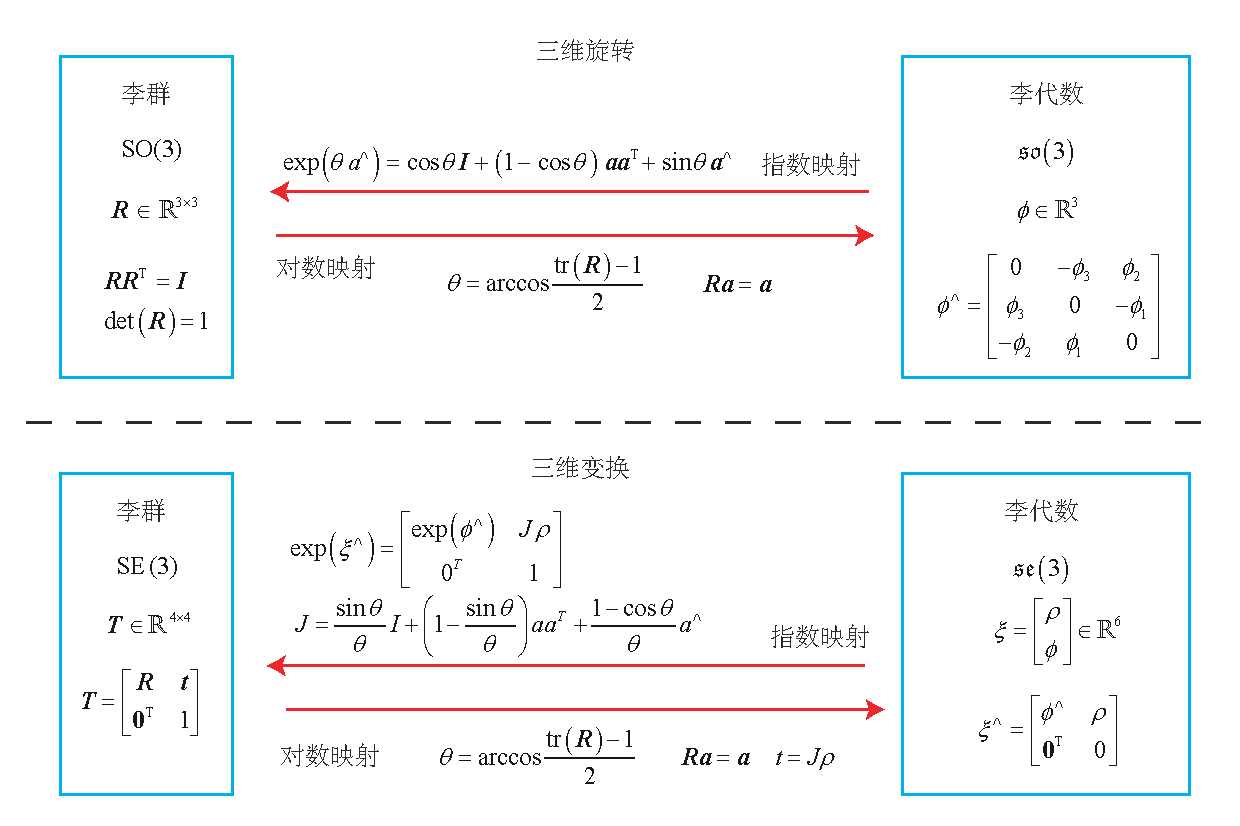
\includegraphics[width=1.0\textwidth]{lieGroup/liegroupandAlgebra.pdf}
	\caption{$\mathrm{SO}(3),\mathrm{SE}(3),\mathfrak{so}(3), \mathfrak{se}(3)$的对应关系。}
	\label{fig:liegroupandAlgebra}
\end{figure}

\clearpage

\section{李代数求导与扰动模型}
\subsection{BCH公式与近似形式}
使用李代数的一大动机是进行优化,而在优化过程中导数是非常必要的信息(我们会在第6讲详细介绍)。下面来考虑一个问题。虽然我们已经清楚了$\mathrm{SO}(3)$和$\mathrm{SE}(3)$上的李群与李代数关系,但是,当在$\mathrm{SO}(3)$中完成两个矩阵乘法时,李代数中$\mathfrak{so}(3)$上发生了什么改变呢?反过来说,当$\mathfrak{so}(3)$上做两个李代数的加法时,$\mathrm{SO}(3)$上是否对应着两个矩阵的乘积?如果成立,相当于:
\[
\exp \left( {\boldsymbol{\phi} _1^ \wedge } \right)\exp \left( {\boldsymbol{\phi} _2^ \wedge } \right) = \exp \left( {{{\left( {{\boldsymbol{\phi} _1} + {\boldsymbol{\phi} _2}} \right)}^ \wedge }} \right) ?
\]

如果$\boldsymbol{\phi}_1, \boldsymbol{\phi}_2$为标量,那显然该式成立;但此处我们计算的是\textbf{矩阵}的指数函数,而非标量的指数。换言之,我们在研究下式是否成立:
\[
	\ln \left( \exp \left( \bm{A} \right) \exp \left( \bm{B} \right) \right) = \bm{A} + \bm{B} \; ?
\]

很遗憾,该式在矩阵时并不成立。两个李代数指数映射乘积的完整形式,由Baker-Campbell-Hausdorff公式(BCH公式)\footnote{ 参见\url{https://en.wikipedia.org/wiki/Baker-Campbell-Hausdorff\_formula}。}给出。由于其完整形式较复杂,我们只给出其展开式的前几项:
\begin{equation}
\ln \left( {\exp \left( \bm{A} \right)\exp \left( \bm{B} \right)} \right) = \bm{A} + \bm{B} + \frac{1}{2}\left[ {\bm{A}, \bm{B}} \right] + \frac{1}{{12}}\left[ {\bm{A},\left[ {\bm{A}, \bm{B}} \right]} \right] - \frac{1}{{12}}\left[ {\bm{B},\left[ {\bm{A},\bm{B}} \right]} \right] +  \cdots 
\end{equation}
其中$[]$为李括号。BCH公式告诉我们,当处理两个矩阵指数之积时,它们会产生一些由李括号组成的余项。特别地,考虑$\mathrm{SO}(3)$上的李代数$\ln { \left( {\exp \left( { \boldsymbol{\phi} _1^ \wedge } \right)\exp \left( {\boldsymbol{\phi} _2^ \wedge } \right)} \right) ^ \vee }$,当$\boldsymbol{\phi_1}$或$\boldsymbol{\phi_2}$为小量时,小量二次以上的项都可以被忽略掉。此时,BCH拥有线性近似表达\footnote{对BCH具体形式和近似表达的具体推导,本书不作讨论,请参考文献\cite{Barfoot2016}。}:
\begin{equation}
 \ln { \left( {\exp \left( { \boldsymbol{\phi} _1^ \wedge } \right)\exp \left( {\boldsymbol{\phi} _2^ \wedge } \right)} \right) ^ \vee } \approx \left\{ 
 \begin{array}{l}
 {\bm{J}_l}{\left( {{\boldsymbol{\phi} _2}} \right)^{ - 1}}{ \boldsymbol{\phi} _1} + {\boldsymbol{\phi} _2} \quad \text{当} \boldsymbol{\phi}_1 \text{为小量},\\
 {\bm{J}_r}{\left( {{\boldsymbol{\phi} _1}} \right)^{ - 1}}{\boldsymbol{\phi} _2} + {\boldsymbol{\phi} _1} \quad \text{当} \boldsymbol{\phi}_2 \text{为小量}.
 \end{array} \right.
\end{equation}

以第一个近似为例。该式告诉我们,当对一个旋转矩阵$\bm{R}_2$(李代数为$\boldsymbol{\phi}_2$)左乘一个微小旋转矩阵$\bm{R}_1$(李代数为$\boldsymbol{\phi} _1$)时,可以近似地看作,在原有的李代数$\boldsymbol{\phi}_2$上加上了一项${\bm{J}_l}{\left( {{\boldsymbol{\phi} _2}} \right)^{ - 1}}{ \boldsymbol{\phi} _1}$。同理,第二个近似描述了右乘一个微小位移的情况。于是,李代数在BCH近似下,分成了左乘近似和右乘近似两种,在使用时我们须注意使用的是左乘模型还是右乘模型。

本书以左乘为例。左乘BCH近似雅可比$\bm{J}_l$事实上就是式~\eqref{eq:lieAlgebraJacobian}~的内容:
\begin{equation} 
{ \bm{J}_l} = \bm{J} = \frac{{\sin \theta }}{\theta } \bm{I} + \left( {1 - \frac{{\sin \theta }}{\theta }} \right) \bm{a} { \bm{a}^\mathrm{T}} + \frac{{1 - \cos \theta }}{\theta }{ \bm{a}^ \wedge}.
\end{equation}

它的逆为:
\begin{equation}
\bm{J}_l^{ - 1} = \frac{\theta }{2}\cot \frac{\theta }{2} \bm{I} + \left( {1 - \frac{\theta }{2}\cot \frac{\theta }{2}} \right) \bm{a} {\bm{a}^\mathrm{T}} - \frac{\theta }{2}{ \bm{a}^ \wedge }.
\end{equation}
而右乘雅可比仅需要对自变量取负号即可:
\begin{equation}
\bm{J}_r(\boldsymbol{\phi}) =\bm{J}_l(-\boldsymbol{\phi}) .
\end{equation}

这样,我们就可以谈论李群乘法与李代数加法的关系了。

为了方便读者理解,我们重新叙述一下BCH近似的意义。假定对某个旋转$\bm{R}$,对应的李代数为$\boldsymbol{\phi}$。我们给它左乘一个微小旋转,记作$\Delta \bm{R}$,对应的李代数为$\Delta \boldsymbol{\phi}$。那么,在李群上,得到的结果就是$ \Delta \bm{R} \cdot \bm{R}$,而在李代数上,根据BCH近似,为$\bm{J}_l^{-1} (\boldsymbol{\phi}) \Delta \boldsymbol{\phi} + \boldsymbol{\phi}$。合并起来,可以简单地写成:
\begin{equation}
\exp \left( {\Delta { \boldsymbol{\phi} ^ \wedge }} \right)\exp \left( {{ \boldsymbol{\phi} ^ \wedge }} \right) = \exp \left( {{{\left( { \boldsymbol{\phi}  + \bm{J}_l^{ - 1}\left( \boldsymbol{\phi}  \right)\Delta \boldsymbol{\phi} } \right)}^ \wedge }} \right).
\end{equation}

反之,如果我们在李代数上进行加法,让一个$\boldsymbol{\phi}$加上$\Delta \boldsymbol{\phi}$,那么可以近似为李群上带左右雅可比的乘法:
\begin{equation}
\exp \left( {{{\left( { \boldsymbol{\phi}  + \Delta \boldsymbol{\phi} } \right)}^ \wedge }} \right) = \exp \left( {{{\left( {{ \bm{J}_l}\Delta \boldsymbol{\phi} } \right)}^ \wedge }} \right)\exp \left( {{ \boldsymbol{\phi} ^ \wedge }} \right) = \exp \left( {{\boldsymbol{\phi} ^ \wedge }} \right)\exp \left( {{{\left( {{\bm{J}_r}\Delta \boldsymbol{\phi} } \right)}^ \wedge }} \right).
\end{equation}

这就为之后李代数上做微积分提供了理论基础。同样地,对于$\mathrm{SE}(3)$,亦有类似的BCH近似:
\begin{equation}
\exp \left( {\Delta {\boldsymbol{\xi} ^ \wedge }} \right)\exp \left( {{ \boldsymbol{\xi} ^ \wedge }} \right) \approx \exp \left( {{{\left( {{ \bm{\mathcal{J}}_l^{-1} }\Delta \boldsymbol{\xi}  + \boldsymbol{\xi} } \right)}^ \wedge }} \right),
\end{equation}
\begin{equation}
\exp \left( {{ \boldsymbol{\xi} ^ \wedge }} \right) \exp \left( {\Delta {\boldsymbol{\xi} ^ \wedge }} \right)  \approx \exp \left( {{{\left( {{ \bm{\mathcal{J}}_r^{-1} }\Delta \boldsymbol{\xi}  + \boldsymbol{\xi} } \right)}^ \wedge }} \right).
\end{equation}

这里$\bm{\mathcal{J}}_l$形式比较复杂,它是一个$6 \times 6$的矩阵,读者可以参考文献\cite{Barfoot2016}中式(7.82)和(7.83)的内容。由于我们在计算中没有用到该雅可比,故这里略去它的实际形式。

\enlargethispage{9pt}
\subsection{$\mathrm{SO}(3)$李代数上的求导}
下面来讨论一个带有李代数的函数,如何关于该李代数求导的问题。该问题有很强的实际背景。在SLAM中,我们要估计一个相机的位置和姿态,该位姿是由$\mathrm{SO}(3)$上的旋转矩阵或$\mathrm{SE}(3)$上的变换矩阵描述的。不妨设某个时刻小萝卜的位姿为$\bm{T}$。它观察到了一个世界坐标位于$\bm{p}$的点,产生了一个观测数据$\bm{z}$。那么,由坐标变换关系知:
%\clearpage
\begin{equation}
\bm{z} = \bm{T} \bm{p} + \bm{w}.
\end{equation}
其中$\bm{w}$为随机噪声。由于它的存在,$\bm{z}$往往不可能精确地满足$\bm{z} = \bm{T} \bm{p}$的关系。所以,我们通常会计算理想的观测与实际数据的误差:
\begin{equation}
\bm{e} = \bm{z} - \bm{T} \bm{p}.
\end{equation}

假设一共有$N$个这样的路标点和观测,于是就有$N$个上式。那么,对小萝卜的位姿估计,相当于是寻找一个最优的$\bm{T}$,使得整体误差最小化:
\begin{equation}
\mathop {\min }\limits_{\bm{T}} J(\bm{T} ) = \sum_{i=1}^{N} \left\| {\bm{z}_i - \bm{Tp}_i} \right\|^2_2.
\end{equation}

求解此问题,需要计算目标函数$J$关于变换矩阵$\bm{T}$的导数。我们把具体的算法留到后面再讲。这里的重点是,\textbf{我们经常会构建与位姿有关的函数,然后讨论该函数关于位姿的导数,以调整当前的估计值}。然而,$\mathrm{SO}(3),\mathrm{SE}(3)$上并没有良好定义的加法,它们只是群。如果我们把$\bm{T}$当成一个普通矩阵来处理优化,那就必须对它加以约束。而从李代数角度来说,由于李代数由向量组成,具有良好的加法运算。因此,使用李代数解决求导问题的思路分为两种:

\begin{enumerate}
	\item 用李代数表示姿态,然后根据李代数加法来对\textbf{李代数求导}。
	\item 对李群\textbf{左乘}或\textbf{右乘}微小扰动,然后对该\textbf{扰动求导},称为左扰动和右扰动模型。
\end{enumerate}

第一种方式对应到李代数的求导模型,而第二种则对应到扰动模型。下面来讨论这两种思路的异同。

\subsection{李代数求导}
首先,考虑$\mathrm{SO}(3)$上的情况。假设我们对一个空间点$\bm{p}$进行了旋转,得到了$\bm{R} \bm{p}$。现在,要计算旋转之后点的坐标相对于旋转的导数,我们非正式地记为\footnote{请注意这里并不能按照矩阵微分来定义导数,这只是一个记号。}:
\[
\frac{{\partial \left( {\bm{Rp}} \right)}}{{\partial \bm{R}}}.
\]
由于$\mathrm{SO}(3)$没有加法,所以该导数无法按照导数的定义进行计算。设$\bm{R}$对应的李代数为$\boldsymbol{\phi}$,我们转而计算\footnote{严格说来,在矩阵微分中,只能求行向量关于列向量的导数,所得结果是一个矩阵。但本书写成列向量对列向量的导数,读者可以认为先对分子进行转置,再对最后结果进行转置。这使得式子变得简洁,不然我们就不得不给每一行的分子加一个转置符号。在这种意义下,可以认为$\mathrm{d}(\bm{Ax})/\mathrm{d}\bm{x} = \bm{A}$。}:
\[ \frac{{\partial \left( {\exp \left( \boldsymbol{\phi} ^ \wedge \right) \bm{p}} \right)}}{{\partial \boldsymbol{\phi} }}. \]

%\clearpage
按照导数的定义,有:
\begin{align*}
\frac{{\partial \left( {\exp \left( {{ \boldsymbol{\phi} ^ \wedge }} \right) \bm{p}} \right)}}{{\partial \boldsymbol{\phi} }} &= \mathop {\lim }\limits_{\delta \boldsymbol{\phi}  \to \bm{0}} \frac{{\exp \left( {{{\left( {\boldsymbol{\phi}  + \delta \boldsymbol{\phi} } \right)}^ \wedge }} \right) \bm{p} - \exp \left( {{\boldsymbol{\phi} ^ \wedge }} \right)\bm{p}}}{{\delta \boldsymbol{\phi} }}\\
& = \mathop {\lim }\limits_{\delta \boldsymbol{\phi}  \to \bm{0}} \frac{{\exp \left( {{{\left( {{\bm{J}_l}\delta \boldsymbol{\phi} } \right)}^ \wedge }} \right)\exp \left( {{\boldsymbol{\phi} ^ \wedge }} \right) \bm{p} - \exp \left( {{\boldsymbol{\phi} ^ \wedge }} \right) \bm{p}}}{{\delta \boldsymbol{\phi} }}\\
&= \mathop {\lim }\limits_{\delta \boldsymbol{\phi}  \to \bm{0}} \frac{{\left( { \bm{I} + {{\left( {{ \bm{J}_l}\delta \boldsymbol{\phi} } \right)}^ \wedge }} \right)\exp \left( {{\boldsymbol{\phi} ^ \wedge }} \right) \bm{p} - \exp \left( {{\boldsymbol{\phi} ^ \wedge }} \right)\bm{p}}}{{\delta \boldsymbol{\phi} }}\\
&= \mathop {\lim }\limits_{\delta \boldsymbol{\phi}  \to \bm{0}} \frac{{{{\left( {{\bm{J}_l}\delta \boldsymbol{\phi} } \right)}^ \wedge }\exp \left( {{\boldsymbol{\phi} ^ \wedge }} \right)\bm{p}}}{{\delta \boldsymbol{\phi} }}\\
&= \mathop {\lim }\limits_{\delta \boldsymbol{\phi}  \to \bm{0}} \frac{{ - {{\left( {\exp \left( {{\boldsymbol{\phi} ^ \wedge }} \right)\bm{p}} \right)}^ \wedge }{\bm{J}_l}\delta \boldsymbol{\phi} }}{{\delta \boldsymbol{\phi}}} =  - {\left( {\bm{Rp}} \right)^ \wedge }{\bm{J}_l}.
\end{align*}

第2行的近似为BCH线性近似,第3行为泰勒展开舍去高阶项后的近似(但由于取了极限,可以写等号),第4行至第5行将反对称符号看作叉积,交换之后变号。于是,我们推导出了旋转后的点相对于李代数的导数:
\begin{equation}
\frac{{\partial \left( { \bm{Rp}} \right)}}{{\partial \boldsymbol{\phi} }} = {\left( { - \bm{Rp}} \right)^ \wedge }{\bm{J}_l}.
\end{equation}

不过,由于这里仍然含有形式比较复杂的$\bm{J}_l$,我们不太希望计算它。而下面要讲的扰动模型则提供了更简单的导数计算方式。

\subsection{扰动模型(左乘)}
另一种求导方式是对$\bm{R}$进行一次扰动$\Delta \bm{R}$,看结果相对于扰动的变化率。这个扰动可以乘在左边也可以乘在右边,最后结果会有一点儿微小的差异,我们以左扰动为例。设左扰动$\Delta \bm{R}$对应的李代数为$\boldsymbol{\varphi}$。然后,对$\boldsymbol{\varphi}$求导,即:
\begin{equation}
\frac{{\partial \left( {\bm{Rp}} \right)}}{{\partial \boldsymbol{\varphi} }} = \mathop {\lim }\limits_{\boldsymbol{\varphi}  \to \bm{0}} \frac{{\exp \left( {{\boldsymbol{\varphi} ^ \wedge }} \right)\exp \left( {{\boldsymbol{\phi} ^ \wedge }} \right)\bm{p} - \exp \left( {{\boldsymbol{\phi} ^ \wedge }} \right)\bm{p}}}{\boldsymbol{\varphi} }.
\end{equation}

该式的求导比上面更为简单:
\begin{align*}
\frac{{\partial \left( {\bm{Rp}} \right)}}{{\partial \boldsymbol{\varphi} }} &= \mathop {\lim }\limits_{\boldsymbol{\varphi}  \to \bm{0}} \frac{{\exp \left( {{\boldsymbol{\varphi} ^ \wedge }} \right)\exp \left( {{\boldsymbol{\phi} ^ \wedge }} \right)\bm{p} - \exp \left( {{\boldsymbol{\phi} ^ \wedge }} \right)\bm{p}}}{ \boldsymbol{\varphi} }\\
&= \mathop {\lim }\limits_{\boldsymbol{\varphi } \to \bm{0}} \frac{{\left( {\bm{I} + {\boldsymbol{\varphi }^ \wedge }} \right)\exp \left( {{\boldsymbol{\phi} ^ \wedge }} \right)\bm{p} - \exp \left( {{\boldsymbol{\phi} ^ \wedge }} \right)\bm{p}}}{\boldsymbol{\varphi} }\\
&= \mathop {\lim }\limits_{\boldsymbol{\varphi}  \to \bm{0}} \frac{{{\boldsymbol{\varphi} ^ \wedge }\bm{Rp}}}{\boldsymbol{\varphi} } = \mathop {\lim }\limits_{\boldsymbol{\varphi}  \to \bm{0}} \frac{{ - {{\left( \bm{Rp} \right)}^ \wedge }\boldsymbol{\varphi} }}{\boldsymbol{\varphi} } =  - {\left( \bm{Rp} \right)^ \wedge }.
\end{align*}

可见,相比于直接对李代数求导,省去了一个雅可比$\bm{J}_l$的计算。这使得扰动模型更为实用。请读者务必理解这里的求导运算,这在位姿估计当中具有重要的意义。

\subsection{$\mathrm{SE}(3)$上的李代数求导}
\label{sec:se3-diff}
最后,我们给出$\mathrm{SE}(3)$上的扰动模型,而直接李代数上的求导就不再介绍了。假设某空间点$\bm{p}$经过一次变换$\bm{T}$(对应李代数为$\boldsymbol{\xi}$),得到$\bm{Tp}$\footnote{请注意为了使乘法成立,$\bm{p}$必须使用齐次坐标。}。现在,给$\bm{T}$左乘一个扰动$\Delta \bm{T} = \exp \left( \delta \boldsymbol{\xi}^\wedge  \right)$,我们设扰动项的李代数为$\delta \boldsymbol{\xi} = [\delta \boldsymbol{\rho}, \delta \boldsymbol{\phi}]^\mathrm{T}$,那么:
\begin{align*}
\frac{{\partial \left( \bm{Tp} \right)}}{{\partial \delta \boldsymbol{\xi}}} &= \mathop {\lim }\limits_{\delta \boldsymbol{\xi}  \to \bm{0}} \frac{{\exp \left( {\delta {\boldsymbol{\xi} ^ \wedge }} \right)\exp \left( {{\boldsymbol{\xi} ^ \wedge }} \right) \bm{p} - \exp \left( {{\boldsymbol{\xi} ^ \wedge }} \right) \bm{p} }}{{\delta \boldsymbol{\xi} }}\\
&= \mathop {\lim }\limits_{\delta \boldsymbol{\xi}  \to \bm{0}} \frac{{\left( { \bm{I} + \delta {\boldsymbol{\xi} ^ \wedge }} \right)\exp \left( {{\boldsymbol{\xi} ^ \wedge }} \right) \bm{p} - \exp \left( {{\boldsymbol{\xi} ^ \wedge }} \right) \bm{p} }}{{\delta {\boldsymbol{\xi} }}}\\
&= \mathop {\lim }\limits_{\delta \boldsymbol{\xi}  \to \bm{0}} \frac{{\delta {\boldsymbol{\xi} ^ \wedge }\exp \left( {{\boldsymbol{\xi} ^ \wedge }} \right) \bm{p}}}{{\delta {\boldsymbol{\xi} }}}\\
&= \mathop {\lim }\limits_{\delta \boldsymbol{\xi}  \to \bm{0}} 
\frac{{\left[ {\begin{array}{*{20}{c}}
			{\delta { \boldsymbol{\phi} ^ \wedge }}&{\delta {\boldsymbol{\rho} }}\\
			{{\bm{0}^\mathrm{T}}}&0
			\end{array}} \right]\left[ {\begin{array}{*{20}{c}}
			{\bm{Rp} + \bm{t}}\\
			1
			\end{array}} \right]}}{{\delta {\boldsymbol{\xi} }}}\\
&= \mathop {\lim }\limits_{\delta \boldsymbol{\xi}  \to \bm{0}} \frac{{\left[ {\begin{array}{*{20}{c}}
			{\delta {\boldsymbol{\phi} ^ \wedge }\left( {\bm{Rp} + \bm{t}} \right) + \delta {\boldsymbol{\rho} }}\\
			\bm{0}^\mathrm{T}
			\end{array}} \right]}}{[\delta\boldsymbol{\rho},\delta \boldsymbol{\phi}]^\mathrm{T}} = \left[ {\begin{array}{*{20}{c}}
	\bm{I} & { - {{\left( {\bm{Rp} + \bm{t}} \right)}^ \wedge }} \\
	{{\bm{0}}}^\mathrm{T} & \bm{0}^\mathrm{T}
	\end{array}} \right] \buildrel \Delta \over = {\left( \bm{Tp} \right)^ \odot }.
\end{align*}

我们把最后的结果定义成一个算符$^\odot$\footnote{我会读作“咚”,像一个石子掉在井里的声音。},它把一个齐次坐标的空间点变换成一个$4 \times 6$的矩阵。此式稍微需要解释的是矩阵求导方面的顺序,假设$\bm{a}, \bm{b}, \bm{x}, \bm{y}$都是列向量,那么在我们的符号写法下,有如下的规则:
\begin{equation}
\frac{\mathrm{\mathrm{d}}\begin{bmatrix}
\bm{a}\\
\bm{b}
\end{bmatrix}}{{\mathrm{d} \begin{bmatrix}
\bm{x}\\
\bm{y}
\end{bmatrix}}} = {\left( \frac{\mathrm{d}[\bm{a},\bm{b}]^\mathrm{T}}{{\mathrm{d}\begin{bmatrix}
\bm{x}\\
\bm{y}
\end{bmatrix}}} \right)^\mathrm{T}} = {{\begin{bmatrix}
{\frac{{\mathrm{d}\bm{a}}}{{\mathrm{d}\bm{x}}}}&{\frac{{\mathrm{d}\bm{b}}}{{\mathrm{d}\bm{x}}}}\\
{\frac{{\mathrm{d}\bm{a}}}{{\mathrm{d}\bm{y}}}}&{\frac{{\mathrm{d}\bm{b}}}{{\mathrm{d}\bm{y}}}}
\end{bmatrix}} ^\mathrm{T}} = {\begin{bmatrix}
{\frac{{\mathrm{d}\bm{a}}}{{\mathrm{d}\bm{x}}}}&{\frac{{\mathrm{d}\bm{a}}}{{\mathrm{d}\bm{y}}}}\\
{\frac{{\mathrm{d}\bm{b}}}{{\mathrm{d}\bm{x}}}}&{\frac{{\mathrm{d}\bm{b}}}{{\mathrm{d}\bm{y}}}}
\end{bmatrix}}
\end{equation}

至此,我们已经介绍了李群李代数上的微分运算。之后的章节中,我们将应用这些知识去解决实际问题。关于李群李代数的某些重要数学性质,我们作为习题留给读者。

\section{实践:Sophus}
\subsection{Sophus的基本使用方法}
我们已经介绍了李代数的入门知识,现在是通过实践演练巩固一下所学知识的时候了。我们来讨论如何在程序中操作李代数。在第3讲中,我们看到Eigen提供了几何模块,但没有提供李代数的支持。一个较好的李代数库是Strasdat维护的Sophus库\footnote{最早提出李代数的是Sophus Lie,这个库就以他的名字命名了。}。Sophus库支持本章主要讨论的$\mathrm{SO}(3)$和$\mathrm{SE}(3)$,此外还含有二维运动$\mathrm{SO}(2), \mathrm{SE}(2)$以及相似变换$\mathrm{Sim}(3)$的内容。它是直接在Eigen基础上开发的,我们不需要安装额外的依赖库。读者可以直接从GitHub上获取Sophus,或者,在本书的代码目录slambook/3rdparty下也提供了Sophus源代码。由于历史原因,Sophus早期版本只提供了双精度的李群/李代数类。后续版本改写成了模板类。模板类的Sophus中可以使用不同精度的李群/李代数,但同时增加了使用难度。在本书第二版中,我们使用\textbf{带模板}的Sophus库。本书的3rdparty中提供的Sophus是\textbf{模板}版本,它应该在你下载本书代码的时候就已经复制下来了。Sophus本身亦是一个cmake工程。想必你已经了解如何编译cmake工程了,这里不再赘述。Sophus库只需编译即可,无须安装。

下面来演示一下Sophus库中的SO(3)和SE(3)运算:

\begin{lstlisting}[language=c++,caption=slambook/ch4/useSophus.cpp]
#include <iostream>
#include <cmath>
#include <Eigen/Core>
#include <Eigen/Geometry>
#include "sophus/se3.hpp"

using namespace std;
using namespace Eigen;

/// 本程序演示sophus的基本用法
int main(int argc, char **argv) {
	// 沿Z轴转90度的旋转矩阵
	Matrix3d R = AngleAxisd(M_PI / 2, Vector3d(0, 0, 1)).toRotationMatrix();
	// 或者四元数
	Quaterniond q(R);
	Sophus::SO3d SO3_R(R);              // Sophus::SO3d可以直接从旋转矩阵构造
	Sophus::SO3d SO3_q(q);              // 也可以通过四元数构造
	// 二者是等价的
	cout << "SO(3) from matrix:\n" << SO3_R.matrix() << endl;
	cout << "SO(3) from quaternion:\n" << SO3_q.matrix() << endl;
	cout << "they are equal" << endl;
	
	// 使用对数映射获得它的李代数
	Vector3d so3 = SO3_R.log();
	cout << "so3 = " << so3.transpose() << endl;
	// hat 为向量到反对称矩阵
	cout << "so3 hat=\n" << Sophus::SO3d::hat(so3) << endl;
	// 相对的,vee为反对称到向量
	cout << "so3 hat vee= " << Sophus::SO3d::vee(Sophus::SO3d::hat(so3)).transpose() << endl;
	
	// 增量扰动模型的更新
	Vector3d update_so3(1e-4, 0, 0); //假设更新量为这么多
	Sophus::SO3d SO3_updated = Sophus::SO3d::exp(update_so3) * SO3_R;
	cout << "SO3 updated = \n" << SO3_updated.matrix() << endl;
	
	cout << "*******************************" << endl;
	// 对SE(3)操作大同小异
	Vector3d t(1, 0, 0);           // 沿X轴平移1
	Sophus::SE3d SE3_Rt(R, t);           // 从R,t构造SE(3)
	Sophus::SE3d SE3_qt(q, t);            // 从q,t构造SE(3)
	cout << "SE3 from R,t= \n" << SE3_Rt.matrix() << endl;
	cout << "SE3 from q,t= \n" << SE3_qt.matrix() << endl;
	// 李代数se(3) 是一个六维向量,方便起见先typedef一下
	typedef Eigen::Matrix<double, 6, 1> Vector6d;
	Vector6d se3 = SE3_Rt.log();
	cout << "se3 = " << se3.transpose() << endl;
	// 观察输出,会发现在Sophus中,se(3)的平移在前,旋转在后.
	// 同样的,有hat和vee两个算符
	cout << "se3 hat = \n" << Sophus::SE3d::hat(se3) << endl;
	cout << "se3 hat vee = " << Sophus::SE3d::vee(Sophus::SE3d::hat(se3)).transpose() << endl;
	
	// 最后,演示一下更新
	Vector6d update_se3; //更新量
	update_se3.setZero();
	update_se3(0, 0) = 1e-4d;
	Sophus::SE3d SE3_updated = Sophus::SE3d::exp(update_se3) * SE3_Rt;
	cout << "SE3 updated = " << endl << SE3_updated.matrix() << endl;
	
	return 0;
}
\end{lstlisting}

该演示程序分为两部分。前半部分介绍$\mathrm{SO}(3)$上的操作,后半部分则为$\mathrm{SE}(3)$。我们演示了如何构造$\mathrm{SO}(3),\mathrm{SE}(3)$对象,对它们进行指数、对数映射,以及当知道更新量后,如何对李群元素进行更新。如果读者切实理解了本讲内容,那么这个程序对你来说应该没有什么难度。为了编译它,请在CMakeLists.txt里添加以下几行:

\begin{lstlisting}[caption=slambook/ch4/useSophus/CMakeLists.txt]
# 为使用 sophus,需要使用 find_package 命令找到它
find_package( Sophus REQUIRED )
include_directories( ${Sophus_INCLUDE_DIRS} )

add_executable( useSophus useSophus.cpp )
\end{lstlisting}

find\_package命令是cmake提供的寻找某个库的头文件与库文件的指令。如果cmake能够找到它,就会提供头文件和库文件所在的目录的变量。在Sophus这个例子中,就是Sophus\_INCLUDE\_DIRS。基于模板的Sophus库和Eigen一样,是仅含头文件而没有源文件的。根据它们,我们就能将Sophus库引入自己的cmake工程了。请读者自行查看此程序的输出信息,它与我们之前的推导是一致的。

\subsection{例子:评估轨迹的误差}
在实际工程中,我们经常需要评估一个算法的估计轨迹与真实轨迹的差异,来评价算法的精度。真实轨迹往往通过某些更高精度的系统获得,而估计估计则是待评价的算法计算得到。上一讲我们演示了如何显示存储在文件中的某条轨迹,本节我们来考虑如何计算两条轨迹的误差。考虑一条估计轨迹$\bm{T}_{\mathrm{esti},i}$和真实轨迹$\bm{T}_{\mathrm{gt},i}$,其中$i=1,\cdots,N$,那么我们可以定义一些误差指标来描述它们之间的差别。

误差指标可以有很多种,常见的有\textbf{绝对轨迹误差}(Absolute Trajectory Error, ATE),形如:
\begin{equation}
\mathrm{ATE}_{\mathrm{all}} = \sqrt{ \frac{1}{N} \sum_{i=1}^N \| \log( \bm{T}_{\mathrm{gt},i}^{-1} \bm{T}_{\mathrm{esti},i} )^{\vee} \|_2^2},
\end{equation}
这实际上是每个位姿李代数的\textbf{均方根误差}(Root-Mean-Squared Error, RMSE)。这种误差可以刻画两条轨迹的旋转和平移误差。同时,也有的文献仅考虑平移误差\cite{Sturm2012},从而可以定义\textbf{绝对平移误差}(Average Translational Error):
\begin{equation}
	\mathrm{ATE}_{\mathrm{trans}} = \sqrt{ \frac{1}{N} \sum_{i=1}^N \| \mathrm{trans}( \bm{T}_{\mathrm{gt},i}^{-1} \bm{T}_{\mathrm{esti},i} ) \|_2^2},
\end{equation}
其中$\mathrm{trans}$表示取括号内部变量的平移部分。因为从整条轨迹上来看,旋转出现误差后,随后的轨迹在平移上也会出现误差,所以两种指标在实际当中都适用。

除此之外,也可以定义相对的误差。例如考虑$i$时刻到$i+\Delta t$时刻的运动,那么相对位姿误差(Relative Pose Error, RPE)可定义为:
\begin{equation}
\mathrm{RPE}_{\mathrm{all}} = \sqrt{ \frac{1}{N-\Delta t} \sum_{i=1}^{N-\Delta t} \| \log \left( \left(\bm{T}_{\mathrm{gt},i}^{-1} \bm{T}_{\mathrm{gt},i+\Delta t} )\right)^{-1} \left(\bm{T}_{\mathrm{esti},i}^{-1} \bm{T}_{\mathrm{esti},i+\Delta t}\right)\right)^{\vee} \|_2^2},
\end{equation}
同样地,亦可只取平移部分:
\begin{equation}
\mathrm{RPE}_{\mathrm{trans}} = \sqrt{ \frac{1}{N-\Delta t} \sum_{i=1}^{N-\Delta t} \| \mathrm{trans} \left( \left(\bm{T}_{\mathrm{gt},i}^{-1} \bm{T}_{\mathrm{gt},i+\Delta t} )\right)^{-1} \left(\bm{T}_{\mathrm{esti},i}^{-1} \bm{T}_{\mathrm{esti},i+\Delta t}\right)\right) \|_2^2}.
\end{equation}

利用Sophus库,很容易实现这部分计算。下面我们演示一下绝对轨迹误差的计算。在这个例子中,我们有groundtruth.txt和estimated.txt两条轨迹,下面的代码将读取这两条轨迹,计算误差,然后显示到3D窗口中。为简洁起见,省略了画轨迹部分的代码,在上一讲中我们已经做过类似的工作。
\begin{lstlisting}[language=c++,caption=slambook/ch4/example/trajectoryError.cpp(部分)]
#include <iostream>
#include <fstream>
#include <unistd.h>
#include <pangolin/pangolin.h>
#include <sophus/se3.hpp>

using namespace Sophus;
using namespace std;

string groundtruth_file = "./example/groundtruth.txt";
string estimated_file = "./example/estimated.txt";

typedef vector<Sophus::SE3d, Eigen::aligned_allocator<Sophus::SE3d>> TrajectoryType;

void DrawTrajectory(const TrajectoryType &gt, const TrajectoryType &esti);

TrajectoryType ReadTrajectory(const string &path);

int main(int argc, char **argv) {
	TrajectoryType groundtruth = ReadTrajectory(groundtruth_file);
	TrajectoryType estimated = ReadTrajectory(estimated_file);
	assert(!groundtruth.empty() && !estimated.empty());
	assert(groundtruth.size() == estimated.size());
	
	// compute rmse
	double rmse = 0;
	for (size_t i = 0; i < estimated.size(); i++) {
		Sophus::SE3d p1 = estimated[i], p2 = groundtruth[i];
		double error = (p2.inverse() * p1).log().norm();
		rmse += error * error;
	}
	rmse = rmse / double(estimated.size());
	rmse = sqrt(rmse);
	cout << "RMSE = " << rmse << endl;
	
	DrawTrajectory(groundtruth, estimated);
	return 0;
}

TrajectoryType ReadTrajectory(const string &path) {
	ifstream fin(path);
	TrajectoryType trajectory;
	if (!fin) {
		cerr << "trajectory " << path << " not found." << endl;
		return trajectory;
	}
	
	while (!fin.eof()) {
		double time, tx, ty, tz, qx, qy, qz, qw;
		fin >> time >> tx >> ty >> tz >> qx >> qy >> qz >> qw;
		Sophus::SE3d p1(Eigen::Quaterniond(qx, qy, qz, qw), Eigen::Vector3d(tx, ty, tz));
		trajectory.push_back(p1);
	}
	return trajectory;
}
\end{lstlisting}

该程序输出的结果为2.207,图像如\autoref{fig:trajectory-compare}所示。读者也以尝试将旋转部分去掉,仅计算平移部分的误差。就这个例子来说,我们事实上已经帮助读者做了一些预处理任务,包括轨迹的时间对齐、外参预估,这些内容现在还没有讲到,我们将在以后的学习中谈论。

\begin{figure}[!ht]
	\centering
	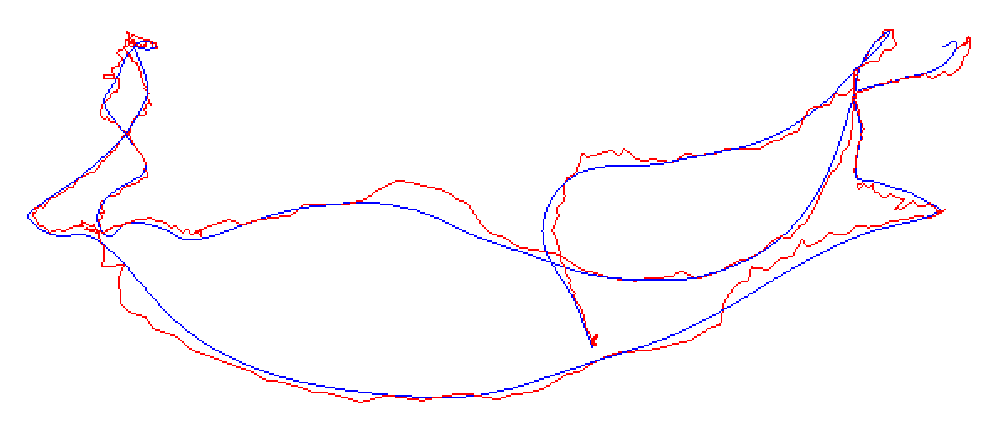
\includegraphics[width=1.0\textwidth]{lieGroup/trajectory-compare.pdf}
	\caption{计算估计轨迹与真实轨迹之间的误差。}
	\label{fig:trajectory-compare}
\end{figure}

\section{\textsuperscript{\ttfamily *}相似变换群与李代数}
最后,我们要提一下在单目视觉中使用的相似变换群$\mathrm{Sim}(3)$,以及对应的李代数$\mathfrak{sim}(3)$。如果你只对双目SLAM或RGB-D SLAM感兴趣,可以跳过本节。

我们已经介绍过单目的尺度不确定性。如果在单目SLAM中使用$\mathrm{SE}(3)$表示位姿,那么由于尺度不确定性与尺度漂移,整个SLAM过程中的尺度会发生变化,这在$\mathrm{SE}(3)$中未能体现出来。因此,在单目情况下我们一般会显式地把尺度因子表达出来。用数学语言来说,对于位于空间的点$\bm{p}$,在相机坐标系下要经过一个\textbf{相似变换},而非欧氏变换:
\begin{equation}\label{key}
\bm{p}' = \left[ {\begin{array}{*{20}{c}}
	{s\bm{R}}&\bm{t}\\
	{{\bm{0}^\mathrm{T}}}&1
	\end{array}} \right] \bm{p}
	= s\bm{R} \bm{p} + \bm{t}.
\end{equation}
在相似变换中,我们把尺度$s$表达了出来。它同时作用在$\bm{p}$的3个坐标之上,对$\bm{p}$进行了一次缩放。与$\mathrm{SO}(3)$、$\mathrm{SE}(3)$相似,相似变换亦对矩阵乘法构成群,称为相似变换群$\mathrm{Sim}(3)$:
\begin{equation}\label{key}
\mathrm{Sim}(3) = \left\{ { \bm{S} = \left[ {\begin{array}{*{20}{c}}
		{s\bm{R}}& \bm{t}\\
		{{\bm{0}^\mathrm{T}}}&1
		\end{array}} \right] \in {\mathbb{R}^{4 \times 4}}} \right\}.
\end{equation}

同样地,$\mathrm{Sim}(3)$也有对应的李代数、指数映射、对数映射等。李代数$\mathfrak{sim}(3)$元素是一个7维向量$\boldsymbol{\zeta}$。它的前6维与$\mathfrak{se}(3)$相同,最后多了一项$\sigma$。
%\clearpage
\begin{equation}
\mathfrak{sim} \left( 3 \right) = \left\{ { \boldsymbol{\zeta} | \boldsymbol{\zeta}  = \left[ \begin{array}{l}
	\boldsymbol{\rho} \\
	\boldsymbol{\phi} \\
	\sigma
	\end{array} \right] \in { \mathbb{R}^7},{ \boldsymbol{\zeta} ^ \wedge } = \left[ {\begin{array}{*{20}{c}}
		{\sigma \bm{I} + {\boldsymbol{\phi} ^ \wedge }}&\boldsymbol{\rho} \\
		{{\bm{0}^\mathrm{T}}}&0
		\end{array}} \right] \in {\mathbb{R}^{4 \times 4}}} \right\}.
\end{equation}

它比$\mathfrak{se}(3)$多了一项$\sigma$。关联$\mathrm{Sim}(3)$和$\mathfrak{sim}(3)$的仍是指数映射和对数映射。指数映射为

\begin{equation}
\exp \left( {{ \boldsymbol{\zeta} ^ \wedge }} \right) = \left[ {\begin{array}{*{20}{c}}
	{{\mathrm{e}^\sigma }\exp \left( {{ \boldsymbol{\phi} ^ \wedge }} \right)}&{ \bm{J}_s \boldsymbol{\rho} }\\
	{{\bm{0}^\mathrm{T}}}&1
	\end{array}} \right].
\end{equation}

其中$\bm{J}_s$形式为
\begin{align*}
%\begin{array}{ll}
{ \bm{J}_s} =& \frac{{{\mathrm{e}^\sigma } - 1}}{\sigma } \bm{I} + \frac{ \sigma {{\mathrm{e}^\sigma }\sin \theta  + \left( {1 - {\mathrm{e}^\sigma }\cos \theta } \right)\theta }}{{{\sigma ^2} + {\theta ^2}}}{\bm{a}^ \wedge }\\
 &+ \left( {\frac{{{\mathrm{e}^\sigma } - 1}}{\sigma } - \frac{{\left( {{\mathrm{e}^\sigma }\cos \theta  - 1} \right)\sigma  + ({\mathrm{e}^\sigma }\sin \theta )\theta }}{{{\sigma ^2} + {\theta ^2}}}} \right){\bm{a}^ \wedge }{\bm{a}^ \wedge }.
%\end{array}
\end{align*}

通过指数映射,我们能够找到李代数与李群的关系。对于李代数$\boldsymbol{\zeta}$,它与李群的对应关系为:
\begin{equation}
s=\mathrm{e}^\sigma, \; \bm{R} = \exp( \boldsymbol{\phi} ^\wedge), \; \bm{t} = \bm{J}_s \boldsymbol{\rho}.
\end{equation}

旋转部分和$\mathrm{SO}(3)$是一致的。平移部分,在$\mathfrak{se}(3)$中需要乘一个雅可比$\bm{\mathcal{J}}$,而相似变换的雅可比更复杂一些。对于尺度因子,可以看到李群中的$s$即为李代数中$\sigma$的指数函数。

$\mathrm{Sim}(3)$的BCH近似与$\mathrm{SE}(3)$是类似的。我们可以讨论一个点$\bm{p}$经过相似变换$\bm{S} \bm{p}$后,相对于$\bm{S}$的导数。同样地,存在微分模型和扰动模型两种方式,而扰动模型较为简单。我们省略推导过程,直接给出扰动模型的结果。设给予$\bm{S} \bm{p}$左侧一个小扰动$\exp( \boldsymbol{\zeta} ^\wedge )$,并求$\bm{S} \bm{p}$对于扰动的导数。因为$\bm{S} \bm{p}$是4维的齐次坐标,$\boldsymbol{\zeta}$是7维向量,该导数应该是$4 \times 7$的雅可比。为了方便起见,记$\bm{Sp}$的前3维组成向量$\bm{q}$,那么:

\begin{equation}
\frac{{\partial \bm{Sp}}}{{\partial \boldsymbol{\zeta} }} = \left[ {\begin{array}{*{20}{c}}
	\bm{I} &{ - {\bm{q}^ \wedge }}& \bm{q} \\
	{{\bm{0}^\mathrm{T}}} & {{ \bm{0}^\mathrm{T}}}&0
	\end{array}} \right].
\end{equation}

关于$\mathrm{Sim}(3)$,我们就介绍到这里。更详细的关于$\mathrm{Sim}(3)$的资料,建议读者参见文献\cite{Strasdat2012a}。


\section{小结}
本讲引入了李群$\mathrm{SO}(3)$和$\mathrm{SE}(3)$,以及它们对应的李代数$\mathfrak{so}(3)$和$\mathfrak{se}(3)$。我们介绍了位姿在它们上面的表达和转换,然后通过BCH的线性近似,就可以对位姿进行扰动并求导了。这给之后讲解位姿的优化打下了理论基础,因为我们需要经常地对某一个位姿的估计值进行调整,使它对应的误差减小。只有在弄清楚如何对位姿进行调整和更新之后,我们才能继续下一步的内容。

本讲的内容可能比较偏理论化,毕竟它不像计算机视觉那样经常有好看的图片可以展示。相比于讲解李群李代数的数学教科书,由于我们只关心实用的内容,所以讲的过程非常精简,速度也相对快了一些。请读者务必理解本讲内容,它是解决后续许多问题的基础,特别是位姿估计部分。

需要一提的是,除了李代数之外,同样也可以用四元数、欧拉角等方式表示旋转,只是后续的处理要麻烦一些。在实际应用中,也可以使用$\mathrm{SO}(3)$加上平移的方式来代替$\mathrm{SE}(3)$,从而回避一些雅可比的计算。

\section*{习题}
\begin{enumerate}
	\item 验证$\mathrm{SO}(3)$、$\mathrm{SE}(3)$和$\mathrm{Sim}(3)$关于乘法成群。
	\item 验证$( \mathbb{R}^3, \mathbb{R}, \times )$构成李代数。
	\item 验证$\mathfrak{so}(3)$和$\mathfrak{se}(3)$满足李代数要求的性质。
	\item 验证性质(4.20)和(4.21)。
	\item 证明:\[
	\bm{R} \bm{p}^\wedge \bm{R}^\mathrm{T} = (\bm{Rp})^\wedge .\]
	\item 证明:\[
	\bm{R} \exp( \bm{p}^\wedge) \bm{R}^\mathrm{T} = \exp( (\bm{Rp})^\wedge ).\] 该式称为$\mathrm{SO}(3)$上的\textbf{伴随}性质。同样地,在$\mathrm{SE}(3)$上亦有伴随性质:
	\begin{equation}
	\bm{T} \exp(\boldsymbol{\xi}^\wedge)\bm{T}^{-1} = \exp \left( \left( \mathrm{Ad}(\bm{T}) \boldsymbol{\xi} \right) ^\wedge \right),
	\end{equation}
	其中:
	\begin{equation}
	\label{eq:adjSE3}
	\mathrm{Ad} ( \bm{T} ) = \left[ {\begin{array}{*{20}{c}}
		\bm{R} &{{ \bm{t} ^ \wedge } \bm{R} }\\
		\bm{0} & \bm{R}
		\end{array}} \right]. 
	\end{equation}
	\item 仿照左扰动的推导,推导$\mathrm{SO}(3)$和$\mathrm{SE}(3)$在右扰动下的导数。
	\item 搜索cmake的find\_package指令是如何运作的。它有哪些可选的参数?为了让cmake找到某个库,需要哪些先决条件?
\end{enumerate}
